%%%%%%%%%%%%%%%%%%%%%%%%%%%%%%%%%%%%%%%%%%%%%%%%%%%%%%%%%%%%%
% ECE 445 SENIOR DESIGN TEMPLATE
%%%%%%%%%%%%%%%%%%%%%%%%%%%%%%%%%%%%%%%%%%%%%%%%%%%%%%%%%%%%%
\documentclass[openbib,letterpaper,10pt]{article}

%%%%%%%%%%%%%%%%%%%%%%%%%%%%%%%%%%%%%%%%%%%%%%%%%%%%%%%%%%%%%
% The preamble starts here.
% You can add other packages that you want to use by using
% \usepackage command in the preamble.
% However, DO NOT change the settings that are already placed
% below unless you really know what you are doing.
%%%%%%%%%%%%%%%%%%%%%%%%%%%%%%%%%%%%%%%%%%%%%%%%%%%%%%%%%%%%%

% some commonly used packages
\usepackage{graphicx}
\usepackage{booktabs}
\usepackage[table]{xcolor}
\usepackage{booktabs}% http://ctan.org/pkg/booktabs
\usepackage{multirow}% http://ctan.org/pkg/multirow
\usepackage{color,soul}
\usepackage{amsmath}
\usepackage{amsthm}
\usepackage{amsfonts}
\usepackage{setspace}
\usepackage{longtable}
\usepackage{url}
\usepackage{float}
\usepackage{caption}
\usepackage[colorlinks=true,linkcolor=black,citecolor=black]{hyperref}
\usepackage[top=1in, bottom=1in, left=1in, right=1in]{geometry}% set the page margins to 1 inch

% use the fancyhdr package to maintain the format of the page numbers,
% which is useful when the text color is changed
\usepackage{fancyhdr}
\fancyhf{}
\renewcommand{\headrulewidth}{1pt}
\renewcommand{\footrulewidth}{0pt}
\fancyfoot[C]{\textcolor{black}{\thepage}}
\fancyhead[L]{
\includegraphics[width=2cm]{University-of-Illinois-logo.jpg}}
\fancyhead[R]{\small{Infantry I.F.F. Proposal - Meyers \& Prince}}

% paralist provides extended list environments
\usepackage{paralist}
\setlength{\plitemsep}{0pt}

% define the color for section and subsection titles
\usepackage{xcolor}
\definecolor{titlecolor}{RGB}{31,73,125}
\definecolor{subtitlecolor}{RGB}{79,129,189}

% tikz/pgf environment for making graphs
\usepackage{tikz}
\usepackage{tikz-timing}[2009/12/09]
\usetikzlibrary{shapes,arrows}
\usetikztiminglibrary[new={char=Q,reset char=R}]{counters}

% change the style of the abstract environment
\usepackage{abstract}
\setlength{\absparsep}{6pt}
\setlength{\absleftindent}{0pt}
\setlength{\absrightindent}{0pt}
\setlength{\abstitleskip}{-18pt}
\renewcommand{\absnamepos}{flushleft}
\renewcommand{\abstractnamefont}{\normalfont\Large\singlespacing\bfseries}
\renewcommand{\abstractname}{\textcolor{titlecolor}{Abstract}}

% change the style of the section and subsection titles
\usepackage{titlesec}
\titleformat{\section}{\color{titlecolor}\Large\bf}{\color{titlecolor}\thesection}{0.8em}{}
\titleformat{\subsection}{\color{subtitlecolor}\large\bf}{\color{subtitlecolor}\thesubsection}{1em}{}
\titleformat{\subsubsection}{\color{subtitlecolor}\normalsize\bf}{\color{subtitlecolor}\thesubsubsection}{1.2em}{}
\titlespacing{\section}{0pt}{0em}{0em}
\titlespacing{\subsection}{0pt}{0em}{0em}
\titlespacing{\subsubsection}{0pt}{0em}{0em}

% change the style of the table of contents
\usepackage{titletoc}
\titlecontents{section}[1.5em]{}{\contentslabel{1.5em}}{\hspace*{-1.5em}}{\titlerule*[0.5pc]{.}\contentspage}
\titlecontents{subsection}[3em]{}{\contentslabel{2.1em}}{\hspace*{-2.1em}}{\titlerule*[0.5pc]{.}\contentspage}
\titlecontents{subsubsection}[5.1em]{}{\contentslabel{2.7em}}{\hspace*{-2.7em}}{\titlerule*[0.5pc]{.}\contentspage}

% command for centering texts in a fixed width table cell
\newcommand{\centpcol}{\leftskip\fill \rightskip\fill}

% command for setting the style of the appendix titles
\newcommand{\setappenstyle}{
	\titleformat{\section}{\color{titlecolor}\Large\bf}{\color{titlecolor}Appendix \Alph{section}}{0.8em}{}
	\titlecontents{section}[0em]{}{Appendix \thecontentslabel \hspace{1em}}{}{\titlerule*[0.5pc]{.}\contentspage}
}

% define the style of the title of the paper
\newcommand{\thetitle}[1]{\title{\begin{LARGE}{\bf #1}\end{LARGE} \color{subtitlecolor}\rule[25pt]{\textwidth}{1pt}}}

% define the style of the author
\newcommand{\theauthor}[3]{
	\author{\vspace{.4in}\\
	\textcolor{black}{By}\\
	#1
	\vspace{1in}\\
	\textcolor{black}{ECE 445 Proposal -} #2\\
	\textcolor{black}{TA:} #3
	\vspace{1in}}
}

% define the style of figure's caption
\newcommand{\figcap}[1]{
	\captionsetup{format=plain,font={small,color=subtitlecolor,singlespacing},margin={0pt,0pt}}
	\caption{\textcolor{subtitlecolor}{#1}}
	\vspace{-5pt}
}

% define the style of table's caption
\newcommand{\tablecap}[1]{
	\captionsetup{format=plain,font={bf,normalsize,singlespacing,color=black},margin={0pt,0pt}}
	\caption{\textcolor{black}{#1}}
	\vspace{-5pt}
}

% define the style of the abstract's page number
\newcommand{\abstractsetting}{
	\pagenumbering{roman}
	\thispagestyle{fancy}
}

\newcommand{\buildtoc}{
	\clearpage
	\singlespacing
	\tableofcontents
	\onehalfspacing
}

% set indentations and the space between paragraghs
\setlength{\parindent}{0pt}
\setlength{\parskip}{8pt}

%%%%%%%%%%%%%%%%%%%%%%%%%%%%%%%%%%%%%%%%%%%%%%%%%%%%%%%%%%%%%
% PREAMBLE ENDS HERE, DOCUMENT STARTS BELOW
%%%%%%%%%%%%%%%%%%%%%%%%%%%%%%%%%%%%%%%%%%%%%%%%%%%%%%%%%%%%%

\begin{document}

% don't change these
\pagestyle{empty}
\doublespacing

% put the title of your project here. DO NOT include the brackets.
\thetitle{{Infantry I.F.F. (Identification Friend or Foe) System}}

% put your names here. seperate by \\. DO NOT include the brackets.
\theauthor{
	{Eric Meyers (emeyer7)}\\
	{Noah Prince (nprince2)}\\
}
{ % put the semester info here. DO NOT include the brackets.
	{Spring 2016}
}
{ % put your TA's name here. DO NOT include the brackets.
	{Braedon Salz}
}

% put the date and project number here. DO NOT include the brackets.
\date{
{February 10th, 2016}\\
Project No. 11
\clearpage
}

% don't change these
\maketitle
\pagestyle{fancy}
\begin{spacing}{1.15}


% build the table of contents. 
\color{black}
\buildtoc
\pagenumbering{gobble}
\section*{Acronyms \& Pre-Requisite Information}
\begin{itemize}
	\item Infantry - branch of a military force that fights on foot.
	\item I.F.F. - Identification Friend or Foe
	\item PWM - Pulse Width Modulation
	\item PCB - Printed Circuit Board
	\item R.F. - Radio Frequency
	\item RTC - Real Time Clock
	\item NEP - Noise-equivalent Power
\end{itemize}
\clearpage
\setcounter{page}{1}
\pagenumbering{arabic}

%SECTION - Introduction
\section{Introduction}
There have been several friendly fire incidents in recorded military history, accounting for an estimated 2\% to 20\% of all casualties in battle\textsuperscript{\cite{USArmy}}. Using attire to identify friend vs enemy is problematic in situations when both sides are clad in the same camouflage pattern, or are obscured by obstacles.

In order to reduce the amount of friendly fire accidents in modern combat, a Infantry I.F.F. (Identification Friend or Foe) will be designed and constructed which will notify a soldier bearing a weapon whether or not their target is friendly.

Several I.F.F. systems exist for aircraft, however not many reliable systems have been constructed to suit infantry that incorporate fast response times and LEDs for indication.

The system will mount to the side of any weapon, send out queries, ask if a target is friendly, and upon receiving a successful (friendly) reply, will notify the operator.

This will be accomplished through a laser transmission system mounted to the rail (weaver mount) of a weapon. If the friendly personnel receives any of this signal (via phototransistors), it will respond with "acknowledgement" that it is friendly. Once the interrogator receives notice that the target is friendly, the dot sight will turn to a different color.

It is important to note that, in order to have a laser communicate "friendly" for a swath the size of a person, there either need to be multiple photodetectors or a large beam from the laser. Because hundreds of photodetectors is not feasible, our design will use optical adjustment to create a large beam. 

Encryption plays a large role in a system like this, and for this reason must be emphasized heavily in the design process. Pulse Width Modulation will be used to transmit a unique I.D. of the interrogator pointing their sights at a friendly target, and upon receiving this laser transmission, the target will respond with an RF signal. This RF Isotropic Signal will be encrypted with a passphrase that is generated using a method similar to a "Time-based one-time password" algorithm.

The benefit of a system like this are the following:
\begin{itemize}
	\item Reduce number of friendly fire accidents during combat \textsuperscript{\cite{Garrison}}
	\item Reduce number of misfires accidents during combat \textsuperscript{\cite{Garrison}}
	\item Notify friendly personnel location of particular friendly target when aiming
	\item Other applications including but not limited to:
	\begin{itemize}
		\item Paintball or Airsoft
		\item Arcade Laser Tag
	\end{itemize}
\end{itemize}

The cost of a system like this will be heavily emphasized throughout the design phase. The team has proposed a schedule dating from February 8th - May 2nd of this semester. This gives the team $\approx$ 3 weeks for design, $\approx$ 7 weeks to assemble, test, and refine, and $\approx$ 3 weeks to document. The cost and schedule are both expanded upon in Section 5 in this document.\\

\clearpage

%SECTION - Design
\section{Design}
\subsection{Block Diagram}
The design of a system like this is very flexible and can be implemented in several ways. The team decided to break this up into two subsystems with individual sub-components. These will be referred to the "friendly interrogator system" and the "friendly target system". 
\begin{enumerate}
	\item Friendly Interrogator System
	\begin{itemize}
		\item Laser Transmission (Transmit Query)
		\item RF Receiver (Receive Acknowledgement)
	\end{itemize}
	\item Friendly Target System
	\begin{itemize}
		\item Photoreceiver (Receive Query)
		\item RF Transmitter (Transmit Acknowledgement)
	\end{itemize}
\end{enumerate}

Below is a block diagram containing all subsystems that will be designed and constructed this semester. The red dotted line is referring to the Laser Subsystem which is essentially a adjustable laser that will reach the desired distance along with a photodetector to detect these signals. The blue dotted line is the R.F. Subsystem which will serve as the "acknowledgement" to the laser signal to notify the interrogator that the target they are pointing their weapon at is friendly. The green dotted line is referring to the Friendly Interrogator and the Friendly Target Subsystem which will be expanded upon in the following pages.
\begin{figure} [H]
	\centering
	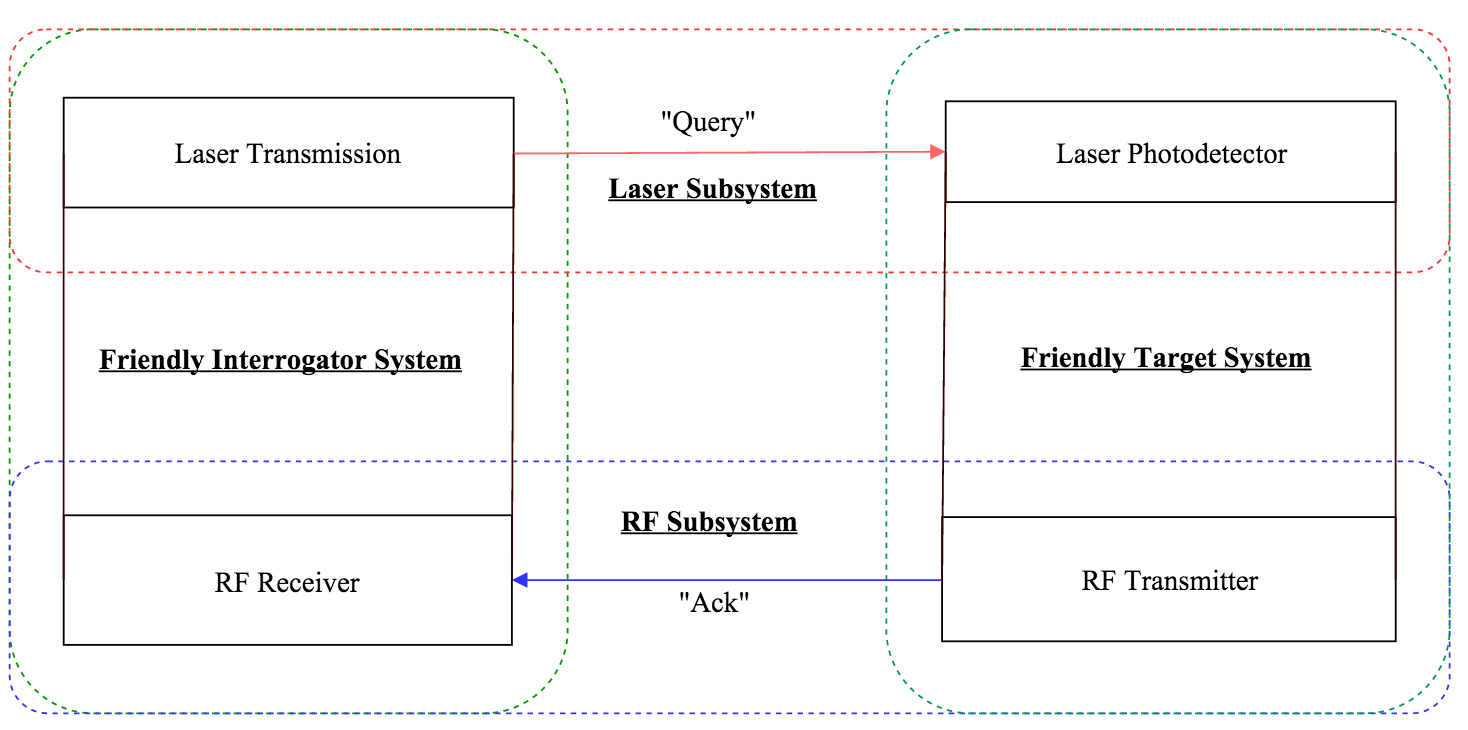
\includegraphics[scale=0.5]{System_Diagram.png}
	\label{fig:system-diagram}
	\caption{I.F.F. Subsystem Diagram}
\end{figure}
\clearpage

\subsection{Block Descriptions}
\subsection*{Friendly Interrogator System}
\begin{figure} [H]
	\centering
	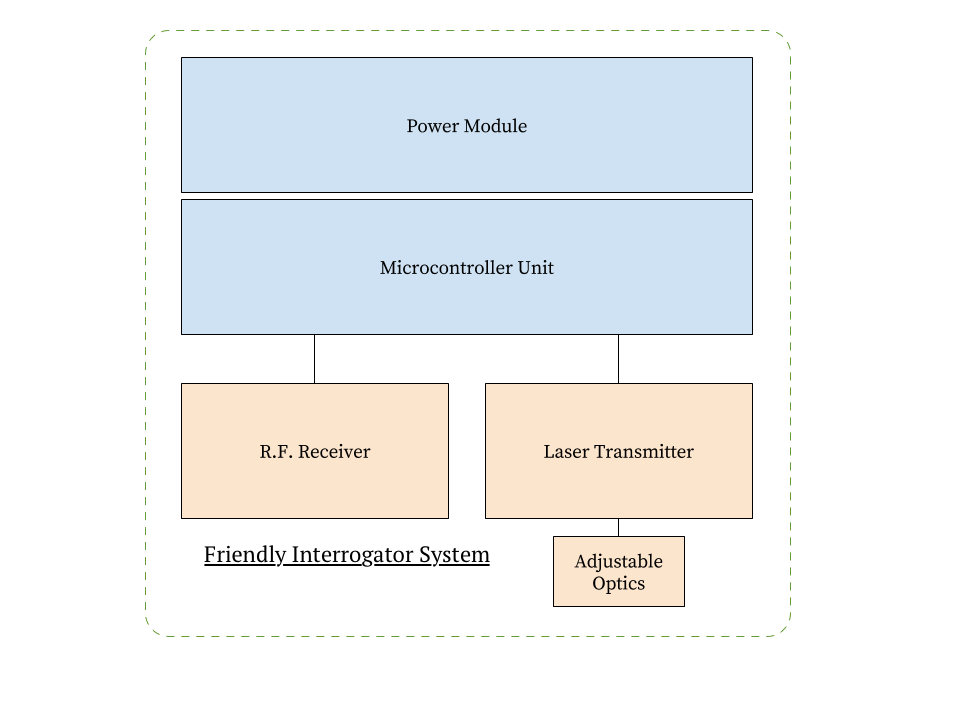
\includegraphics[scale=0.35]{Interrogator_Diagram.png}
	\label{fig:system-diagram}
	\vspace{-10mm}
	\caption{Interrogator System Diagram}
\end{figure}

\subsection*{{\normalsize Laser Transmission}}
\begin{itemize}
	\item Optical adjustment to achieve:
	\begin{itemize}
		\item Short Range (Close Quarters) : 0 - 50 m
		\item Medium Range (Urban Setting) : 50 - 150 m
		\item Long Range : 150 - 300 m
	\end{itemize}
	\item At the extreme of each range, the diameter of the light spot from the laser should be 5-6ft; around the size of a person. 
	\item P.W.M Signal to transmit signal attached with a unique I.D. of interrogator.
		\begin{itemize}
			\item Ability to adjust duty cycle to transmit information 
			\item Preamble followed by unique I.D. of transmitter
		\end{itemize}
\end{itemize}

 \subsection*{{\normalsize  R.F. Receiver}}
\begin{itemize}
	\item Receives "acknowledgement" signal from friendly target
	\item Must have ability to verify passphrase with common clock (Real Time Clock - RTC)
	\item If successful (i.e. system identifies target as friendly), then indicator (LED) will change color from red to green.
\end{itemize}
 
 \subsection*{Friendly Target System}
 
 \begin{figure} [H]
 	\centering
 	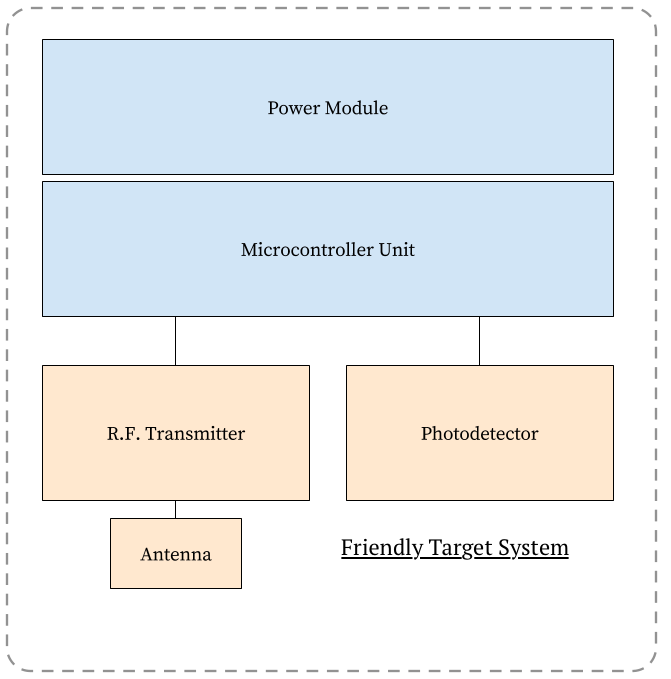
\includegraphics[scale=0.35]{Target_Diagram.png}
 	\label{fig:system-diagram}
 	\vspace{-10mm}
 	\caption{Target System Diagram}
 \end{figure}
 
\subsection*{{\normalsize Laser Photodetector}}

\begin{itemize}
	\item Couse staff and resources provided on Wiki will help narrow down options in the design phase.
	\begin{itemize}
		\item https://courses.engr.illinois.edu/ece445/wiki/?n=Topics.LaserDiodeAndPhotodiodeIntroduction
	\end{itemize}
	\item Photodiode that must be engineered to receive the wavelength and intensity of the laser transmission at maximum range. 
	\item Photodiodes will be mounted on the wearer's helmet, weapon, and/or chest to detect incoming transmissions.
\end{itemize}
 
 \subsection*{{\normalsize  R.F. Transmitter}}
  \begin{itemize}
  	\item Isotropic R.F. Radiator to acknowledge query sent by laser on interrogator
  	\item Ability to reach up to 300 m 
  	\item Encrypted Passphrase
  	\begin{itemize}
  		\item Password generated based off of common clock (RTC)
  		\item Clocks will need to be synced with a common clock source periodically
  	\end{itemize}
  \end{itemize}
 

  \clearpage


%SECTION - Requirements and Verification
\section{Requirements and Verification}


The requirements for this semester are as follows: 
\begin{figure} [H]
	\centering
	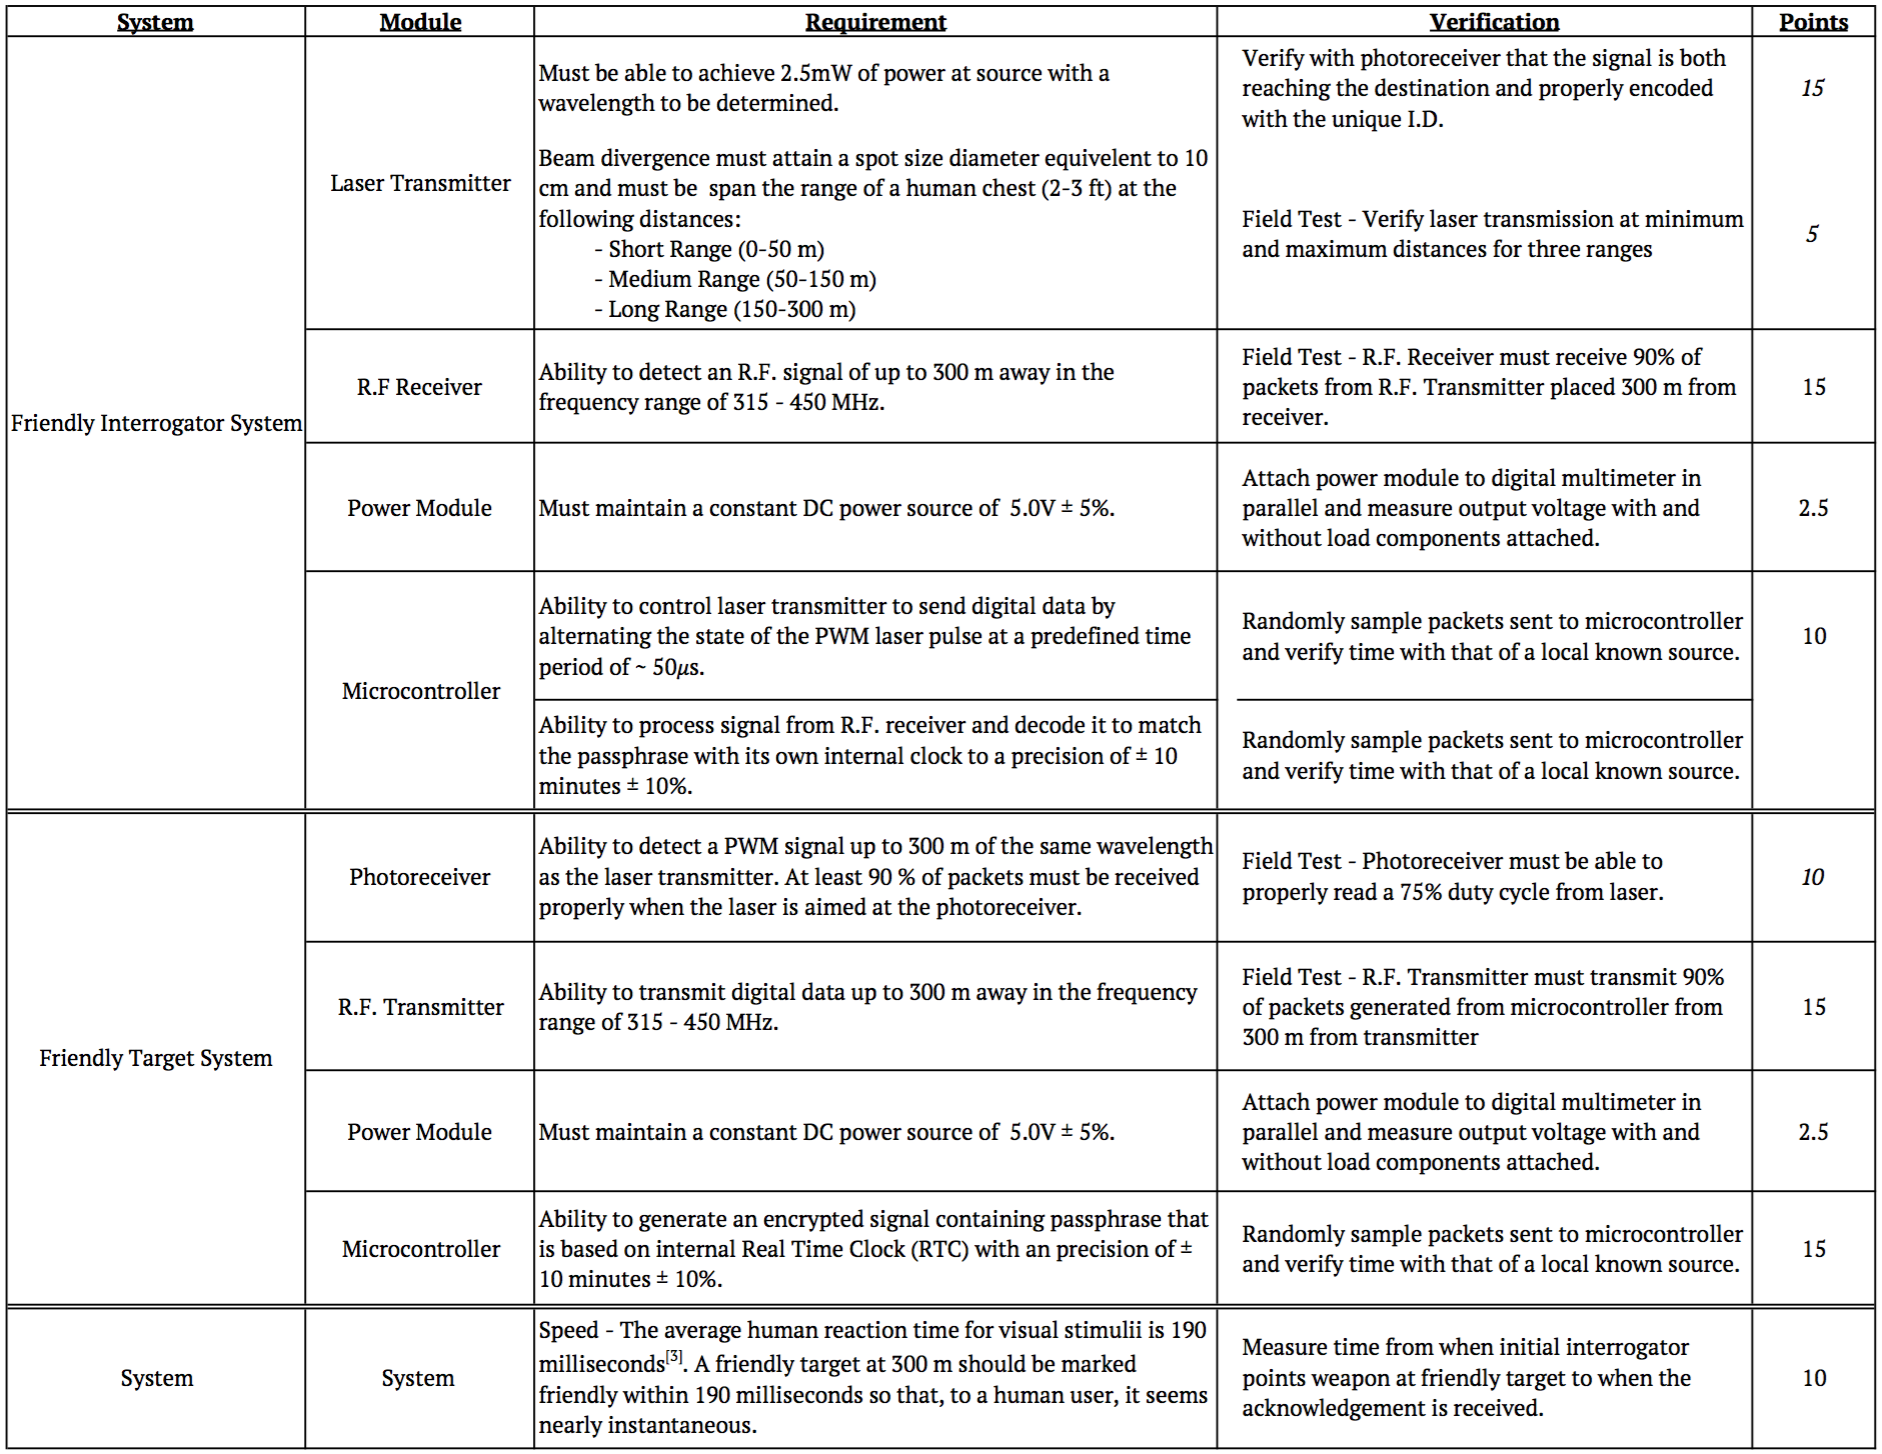
\includegraphics[scale=0.45]{Requirements-Verification-Table.png}
	\label{fig:brequirements-table}
	\caption{Requirements and Verfication Table}
\end{figure}

%SECTION - Tolerance Analysis
\section{Tolerance Analysis}
The signal transmission from the friendly interrogator to the friendly target will be a critical aspect of this project. The extremes of this transmission must be tested; ensuring that it has bot the range and signal span required. 

Capturing these requirements, the team must transmit a signal to a photo-detector at the following ranges:
		\begin{itemize}
			\item Short Range (0 - 50 m)
			\item Medium Range (50 - 150 m)
			\item Long Range (150 - 300 m)
		\end{itemize}

The team should then verify that the signal was received and processed by the MCU. Furthermore, the team should verify that the signal spans the width of a human chest. More concretely, that a sighted-in laser transmitter can be aimed at any point within 2.5 - 3 feet of the receiver and still register friendly. 

The team must transmit a signal over a distance of 300 meters that has the ability to be accurately received by a photo-detector and processed by an MCU. 

Test Procedure:
 
\begin{itemize}
	\item Mount the receiver 300 m downrange of the transmitter
	\item Aim the laser transmitter directly at the receiver, using a mount (like a vice grip) to keep it stable. 
	\item Verify the signal is received.
	\item Aim and verify the signal is also received when aiming 2.5ft to the right, top, and bottom of the receiver. 
	\item Repeat these steps for 50 m and 150 m. 
\end{itemize}

Ensuring that the laser can broadcast over this distance, with divergence, requires a careful selection of parts; including a sensitive photodiode and a powerful laser. 

Because photodiodes are generally cheaper and consume less power than lasers, our starting point for selection criteria was to choose a sensitive photodiode. As such, we have selected the PIN photodiode. 

With photodiodes, Noise-equivalent Power (NEP) is a measure of the incident power required to generate a response signal equal to the noise level of a detector system. Detectivity is the reciprocal of the NEP normalized for the active area of the photodiode.\textsuperscript{\cite{Microphotonics}}. The best photodiode, then, will have the highest detectivity for the infrared wavelength.  

\begin{figure} [H]
	\centering
	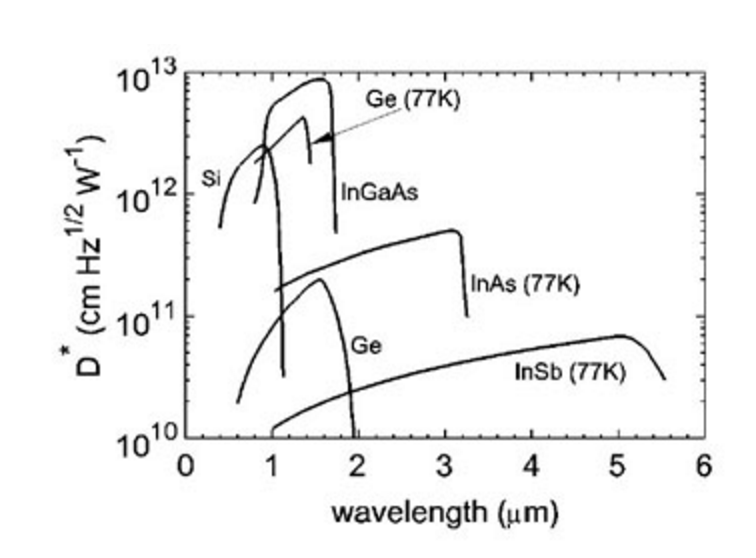
\includegraphics[scale=0.4]{detectivity-table.png}
	\label{fig:detectivity-table}
	\caption{Specific Detectivity for Photodetector Materials \textsuperscript{\cite{Optical}} \label{fig:detectivity-table}}
\end{figure}

Figure \ref{fig:detectivity-table} illustrates the specific detectivity ranges of photodiodes. The interrogation laser is in the infrared range; therefore, the matching photodiode is of type InGaAs. Using this type of photodiode, the detectivity is between $10^{12}$ and $10^{13}$ $\frac{Hz^{\frac{1}{2}}}{W}$. 

The equation to get the NEP from the detectivity is $\frac{A^{1/2}}{NEP}$. The NEP, then, for a 5mm photodiode is $\frac{\sqrt{.0025^2 * \pi}}{10^{12}} = 4.431 * 10^{-15} \frac{W}{Hz^{1/2}}$. Assuming we are operating in the IR wavelength, lets say the frequency is $4*10^{14} Hz$. This means the amount of power incident on the photodiode to cancel noise is $\sqrt{4*10^{14}Hz} * 4.431 * 10^{-15} \frac{W}{Hz^{1/2}} = 8.862*10^{-8} W$. 

Taking the power to include the area of the photodiode, it takes $\frac{8.862*10^{-8}}{.0025^2 * \pi} \approx 0.0045 \frac{W}{m^2}$ for a signal to cancel out the noise. Broadcasting a PWM signal means producing a signal that registers as more than noise. As such, we will up the theoretical required energy by $100\%$. Assume $0.009 \frac{W}{m^2}$ is necessary to broadcast a PWM signal. \\

Now, assume the laser comes out of a diverging lens in the form of a cone. Neglecting dissipation from light reflecting off of air, we can assume that the loss in power per unit area of the laser happens with respect to the area of the light spot. That is, a 5mW laser diverged to a 5 ft diameter will have much less power per area than a concentrated 5mW laser with an inch diameter.

The laser must cover a diameter of 5.5ft (1.6764 m) at 300 m. Let $P$ be the laser power needed. $\frac{P}{0.8382^2* \pi} = .009  \frac{w}{m^2}$

This means the required power, $P$, is 18 milliwatts. 

Please note that the work being performed in the tolerance analysis sections takes up a total of 30 points in the requirements/verification table. 


%SECTION - Cost and Schedule
\section{Cost \& Schedule}
The schedule and budget of this project will be analyzed in the sections below.

\subsection{Schedule}
Please refer to Figure \ref{fig:timeline} for the brief timeline of this project highlighting the milestones and approximate duration of each phase. Refer to Figure \ref{fig:schedule} for an extended week-to-week description of what the team wishes to accomplish over the duration of the semester.


\begin{figure} [H]
	\centering
	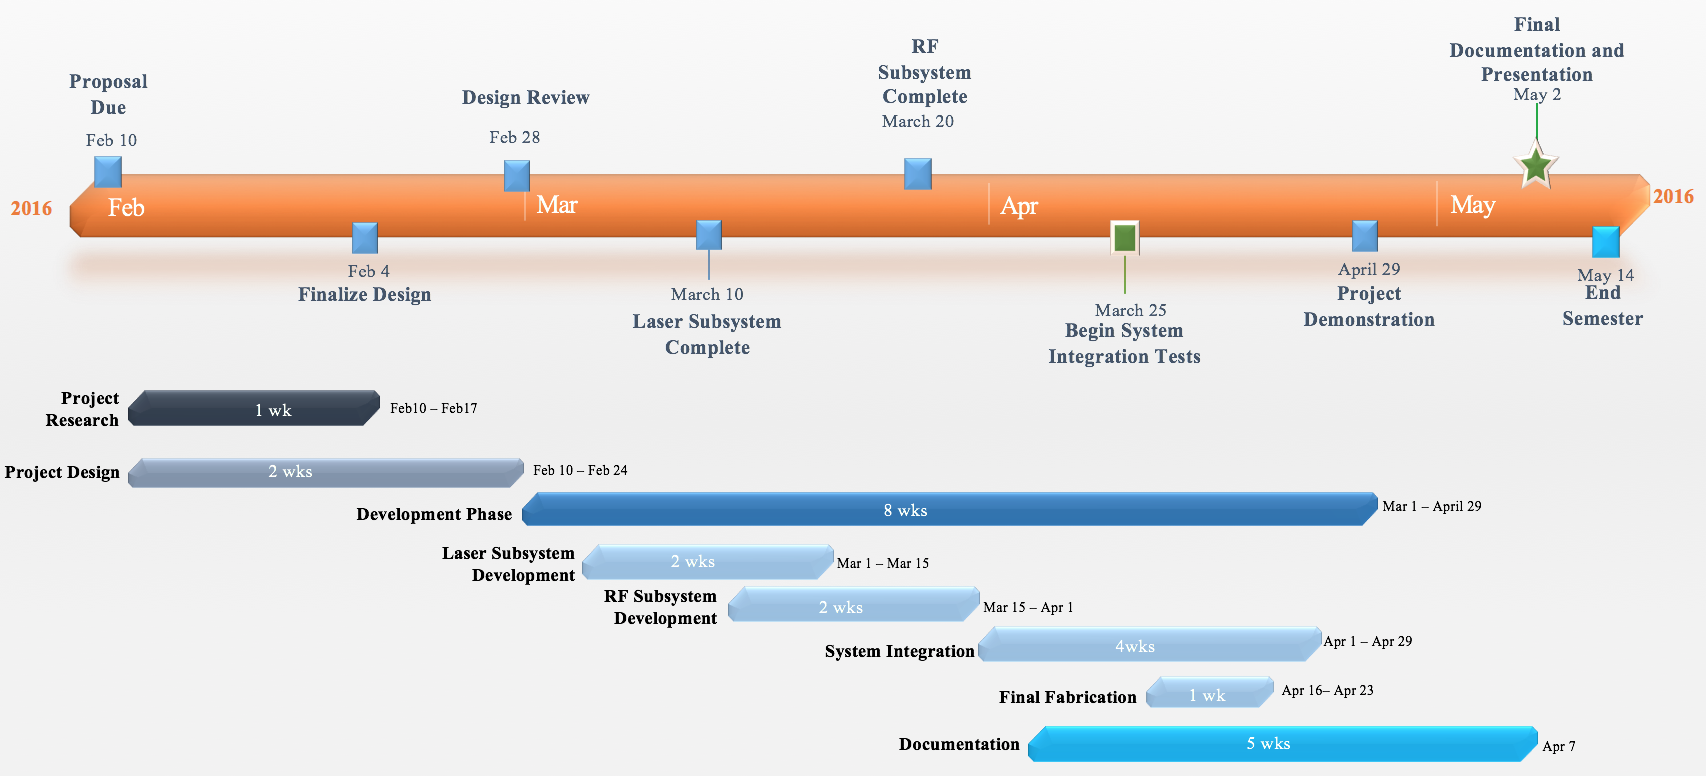
\includegraphics[scale=0.5]{Timeline.png}
	\label{fig:timeline}
	\caption{Timeline with Milestones\label{fig:timeline}}
\end{figure}

\begin{figure} [H]
	\centering
	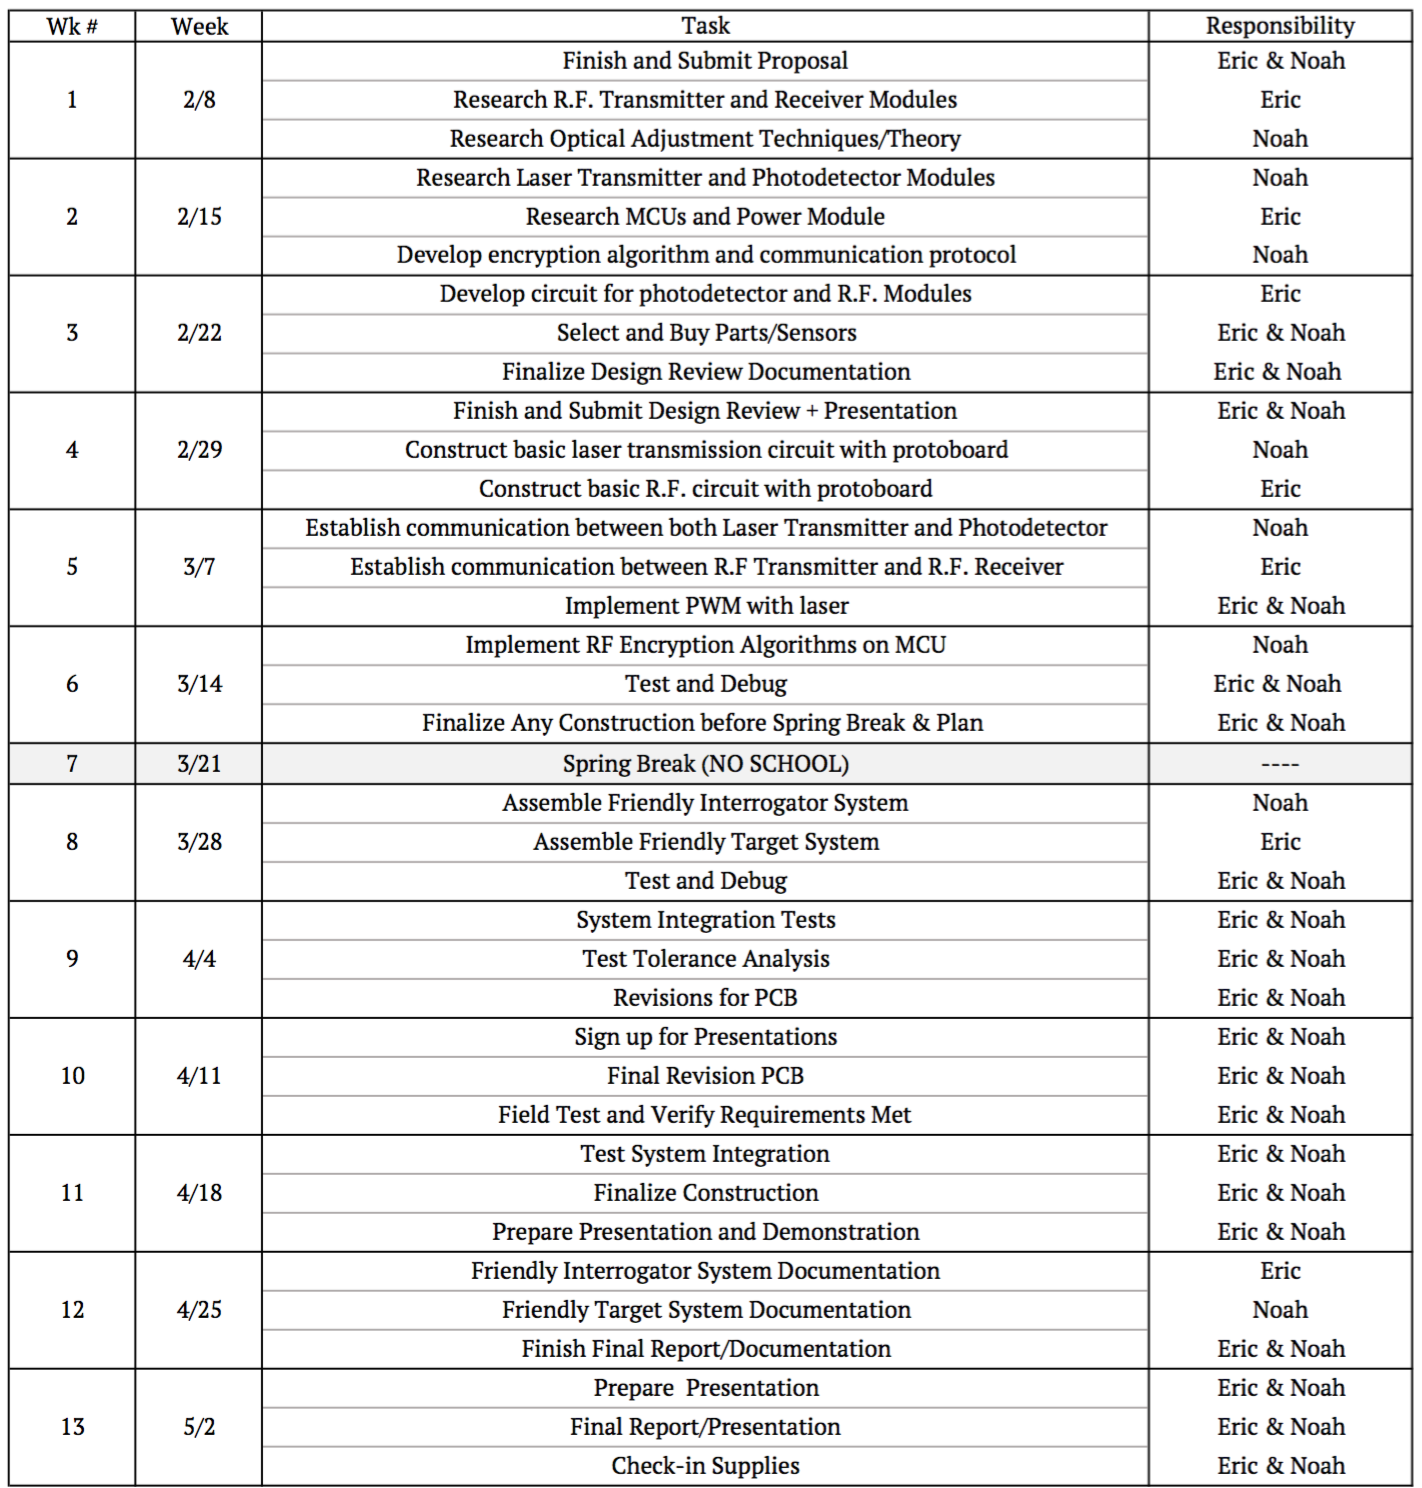
\includegraphics[scale=0.65]{Schedule_Extended.png}
	\caption{Extended Schedule Week-by-Week\label{fig:schedule}}
\end{figure}


\subsection{Cost \& Labor}
This appears to be a fairly demanding Senior Design project. The team has approximately 12 weeks to design, implement, and fabricate this project. Each member of the team will likely work at least 15-20 hours/week on the project. This means $\approx$ 200 hours per team member for the semester. 

The following is a rough cost analysis of the project: 
\begin{figure} [H]
	\centering
	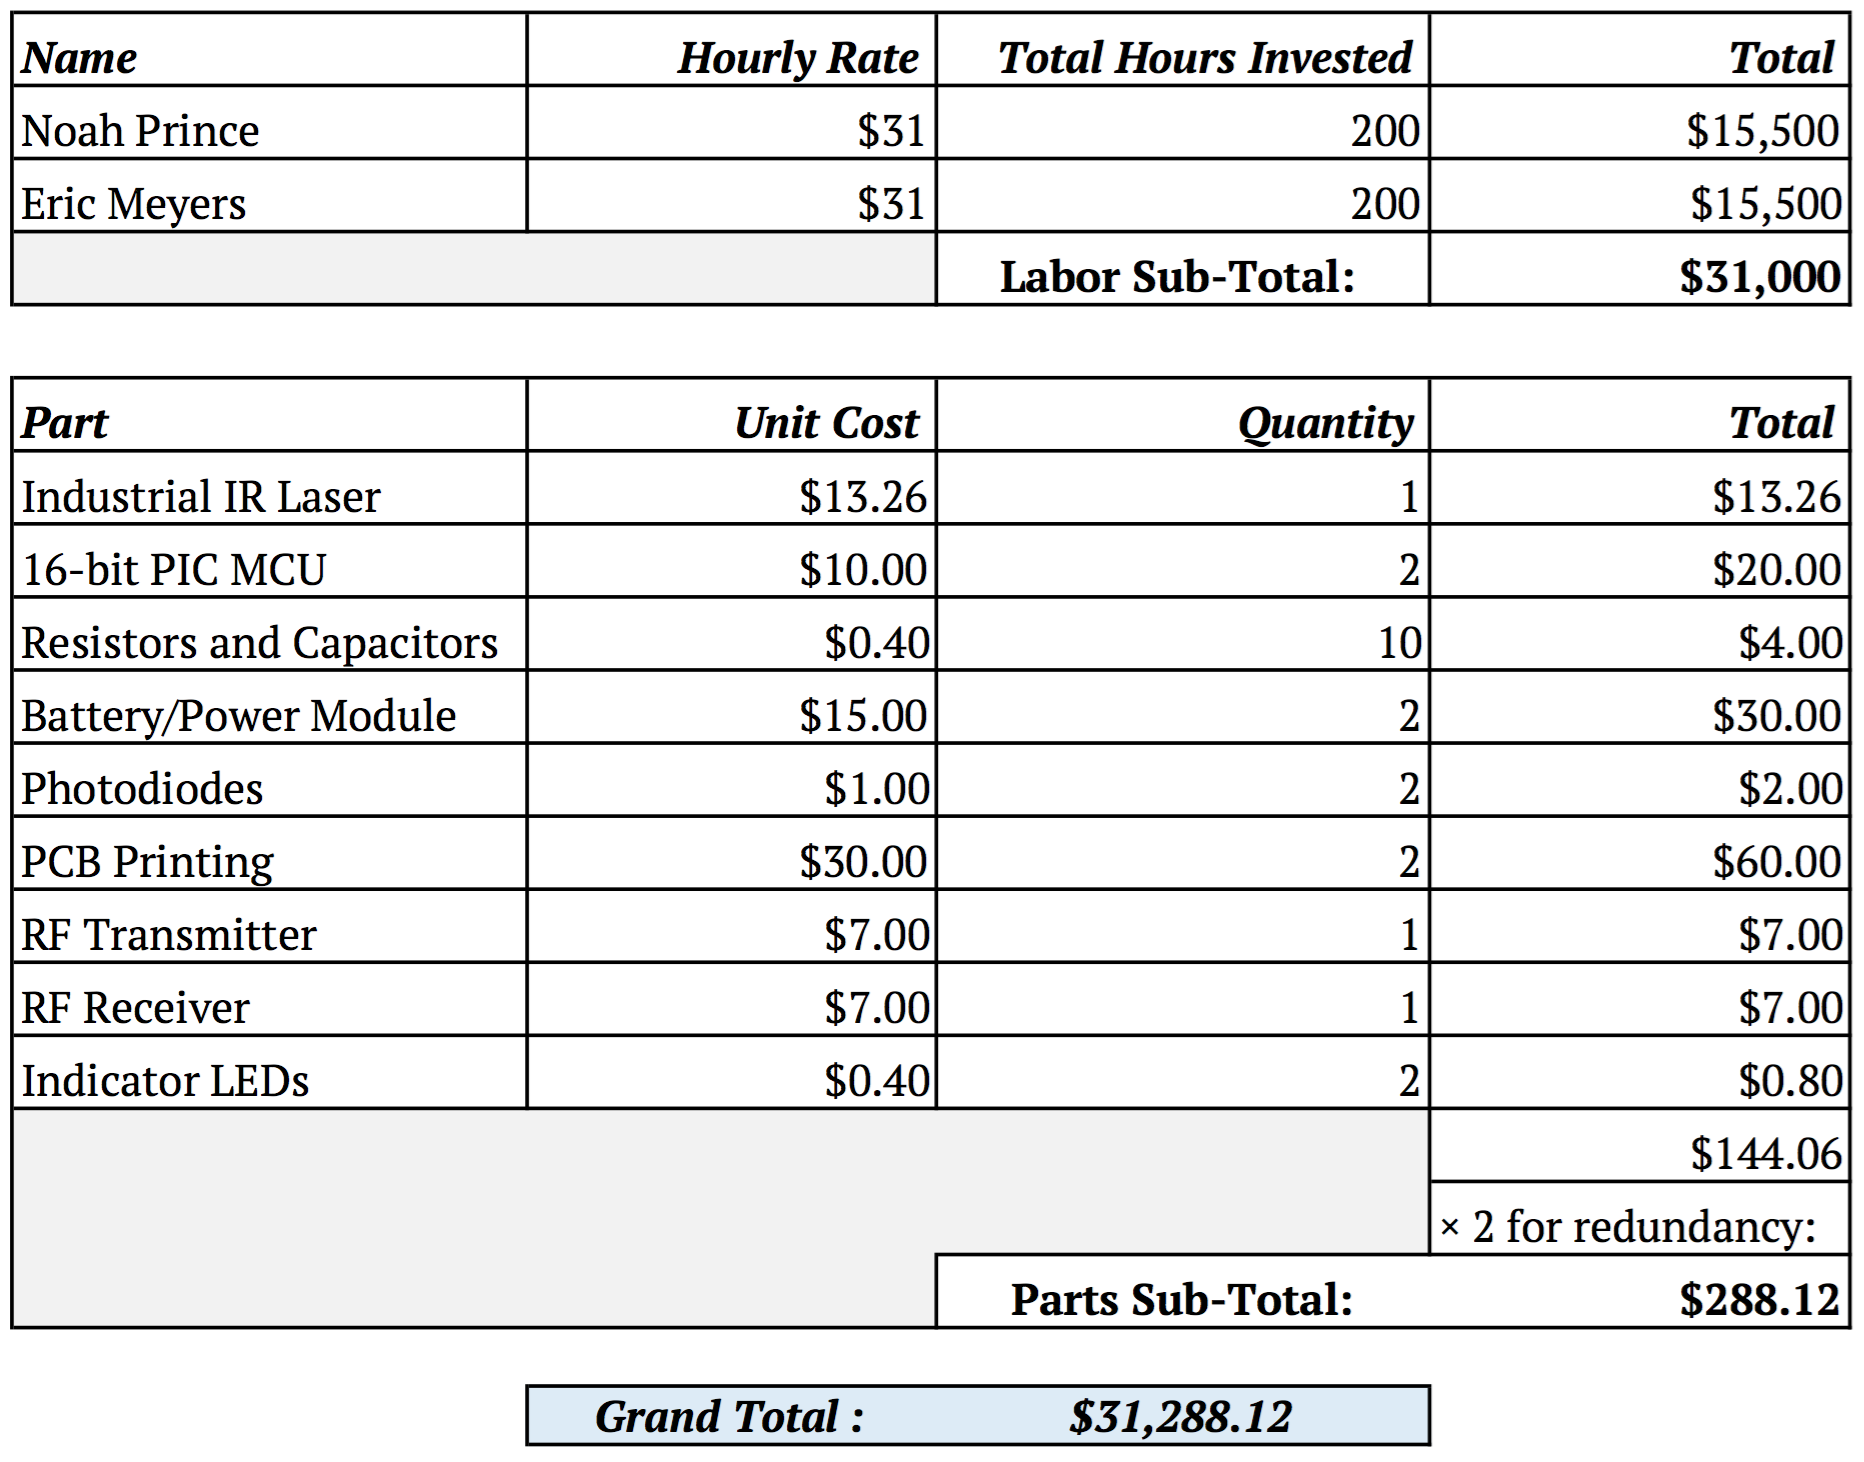
\includegraphics[scale=0.4]{cost-labor-table.png}
	\label{fig:brequirements-table}
	\caption{Labor and Cost Analysis Table}
\end{figure}
\vspace{-5mm}
The labor cost was calculated as follows:

\begin{center}
	Labor Cost = Worker Salary (\$/hour) x 2.5 x Time (Hours) Invested In Project
\end{center}

The parts estimate is not final by any means, this is just a rough estimate of what the team can expect during the design review.  

\bibliographystyle{IEEE_ECE}
% include the BibTex file here to build reference
\bibliography{Citations}\addcontentsline{toc}{section}{Reference}

\clearpage
\end{spacing}
\end{document}

